\documentclass[pdf]{beamer}
\mode<presentation>{
	\usetheme{Ilmenau}
	
}
\usecolortheme{dolphin}
%\usepackage{color,graphicx}
%\usepackage{mathrsfs,amsbsy}
\usepackage{bm}
\usepackage{booktabs}
\usepackage[UTF8,noindent]{ctexcap}
\usepackage{amssymb}
\usepackage{amsmath}
\usepackage{amsfonts}
\usepackage{array}
\usepackage{fancyhdr}
\usepackage{hhline}
%\usepackage[unicode, bookmarksnumbered]{hyperref}	% 启动超链接和 PDF 文档信息所需
\usepackage{graphicx}
\usepackage{amsthm}
\usepackage{enumerate}
\usepackage[mathscr]{eucal}
\usepackage{mathrsfs}
\usepackage{verbatim}
\usepackage{wrapfig}
\usepackage{pgfplots}
%\usepackage{geometry} %调整页面的页边距
\usepackage{pifont}
%\geometry{left=2.5cm,right=2.5cm,top=2cm,bottom=2.5cm}%具体的页边距设置
%\usepackage[notcite,notref]{showkeys}

% showkeys  make label explicit on the paper

%\makeatletter
%\@namedef{subjclassname@2010}{%
%  \textup{2010} Mathematics Subject Classification}
%\makeatother
\usepackage{tikz-cd}
\usepackage{tikz}
\usetikzlibrary{shapes.geometric, arrows}
\numberwithin{equation}{section}
\usepackage[OT2,T1]{fontenc}
\DeclareSymbolFont{cyrletters}{OT2}{wncyr}{m}{n}
\DeclareMathSymbol{\Sha}{\mathalpha}{cyrletters}{"58}
\theoremstyle{plain}
%\newtheorem{theorem}{Theorem}[section]
%\newtheorem{lemma}[theorem]{Lemma}
\newtheorem{proposition}[theorem]{Proposition}
%\newtheorem{corollary}[theorem]{Corollary}
\newtheorem{claim}[theorem]{Claim}
\newtheorem{defn}[theorem]{Definition}
%\newtheorem{example}[theorem]{Example}

\theoremstyle{plain}
\newtheorem{exercise}{Exercise}[section]

\theoremstyle{plain}
\newtheorem{thmsub}{Theorem}[subsection]
\newtheorem{lemmasub}[thmsub]{Lemma}
\newtheorem{corollarysub}[thmsub]{Corollary}
\newtheorem{propositionsub}[thmsub]{Proposition}
\newtheorem{defnsub}[thmsub]{Definition}
\newtheorem{conj}[theorem]{Conjecture}

%\numberwithin{equation}{section}


\theoremstyle{remark}
\newtheorem{remark}[theorem]{Remark}
\newtheorem{remarks}{Remarks}
\newtheorem{ex}[theorem]{Exercise}
\newtheorem{question}[theorem]{Question}

\newcommand*{\thick}[1]{\text{\boldmath$#1$}}
\newcommand*{\cir}[1]{\;$\ding{19#1}$\;}%临时使用
\newcommand*{\norm}[1]{\lVert#1\rVert}
%\renewcommand\thefootnote{\fnsymbol{footnote}}
%dont use number as footnote symbol, use this command to change


\DeclareMathOperator{\supp}{supp}
\DeclareMathOperator{\dist}{dist}
\DeclareMathOperator{\vol}{vol}
\DeclareMathOperator{\diag}{diag}
\DeclareMathOperator{\tr}{tr}
\DeclareMathOperator{\cha}{\operatorname{char}}
\DeclareMathOperator{\Proj}{\operatorname{Proj}}
\DeclareMathOperator{\rank}{\operatorname{rank}}
\DeclareMathOperator{\Ker}{\operatorname{Ker}}
\DeclareMathOperator{\coker}{\operatorname{Coker}}
\DeclareMathOperator{\Img}{\operatorname{Im}}
\DeclareMathOperator{\tor}{\operatorname{tor}}
\newcommand{\Hom}{\operatorname{Hom}}
\newcommand{\Spec}{\operatorname{Spec}}
\newcommand{\Pic}{\operatorname{Pic}}
\newcommand{\Jac}{\operatorname{Jac}}
\newcommand{\MaxSpec}{\operatorname{MaxSpec}}
\newcommand{\End}{\operatorname{End}}
\newcommand{\Mod}{\operatorname{\textbf{Mod}}}
\newcommand{\Gal}{\operatorname{Gal}}
\newcommand{\Grp}{\operatorname{\textbf{Grp}}}
\newcommand{\Set}{\operatorname{\textbf{Set}}}
\newcommand{\Stab}{\operatorname{Stab}}
\newcommand{\ord}{\operatorname{ord}}
\setcounter{tocdepth}{1}




\title{椭圆曲线的理论}
\subtitle{\hspace{5cm}——以Mordell定理为例}
\author{周潇翔}
\institute[USTC]{University of Science and Technology of China}
\date{\today}
\subject{数学基础方向介绍}
\keywords{基础数学,介绍}

\begin{document}
	\begin{frame}
	\titlepage
\end{frame}
\begin{frame}
\begin{abstract}
	\hspace*{20pt}在这份报告中,我们给出
	\begin{itemize}
		\item 对象:椭圆曲线;
		\item 定理:Mordell定理;
		\item 介绍:BSD猜想.
	\end{itemize}
\hspace*{20pt}由于是简要的报告,本人不会具体地深入定理的证明细节,如有需要请参考附件.

\hspace*{20pt}这份报告只花了3-4小时的准备,必有诸多谬误与不当之处,还请谅解.
\end{abstract}

\end{frame}

\begin{frame}{目录}
\tableofcontents
\end{frame}

\section{熟知的代数数论结论}
\begin{frame}{目录}
\tableofcontents[currentsection]
\end{frame}
\begin{frame}[fragile]{理想类群与单位群}
\begin{theorem}\label{thm:idealclass}
	\hspace*{20pt}设$K$为数域,对代数整数环$\mathcal{O}_K$,其理想类群$Cl(K)$
	为有限群,且单位群$\mathcal{O}_K^{\times}$为有限生成群.
\end{theorem}	
	用正合列表示其中的关系.
	\begin{equation*}\label{eq:exactAN}
	\begin{tikzcd}
	0 \arrow[r] & \mathcal{O}_K^{\times} \arrow[r] & K^{\times} \arrow[r, "v"] & \bigoplus\limits_{\mathfrak{p} \in M_K^{0}}\mathbb{Z} \arrow[r] & Cl(K) \arrow[r] & 0
	\end{tikzcd}	
	\end{equation*}
	
	%将$K$视为$\Spec \mathcal{O}_K$上的有理函数空间, $\bigoplus_{\mathfrak{p} \in M_K^{0}}\mathbb{Z}$视为$\Spec \mathcal{O}_K$的除子群,则$v$给出了有理函数(除$0$外)所对应的除子,称为主除子, $Cl(K)$在这个意义下成为$\Spec \mathcal{O}_K$上的Picard群.而对$\mathcal{O}_K^{\times}$,就像黎曼面上的常值函数空间一样,所对应的除子均为$0$.

\end{frame}
\begin{frame}{赋值理论}
\hspace*{20pt}设$L/K$为数域的扩张,则自然有对应环素谱之间的满射:$\pi:\Spec \mathcal{O}_L \longrightarrow \Spec \mathcal{O}_K$.设$\mathfrak{p} \in \Spec \mathcal{O}_K\smallsetminus \{(0)\}$,则我们对$\mathcal{O}_L$的素理想$\mathfrak{p}\mathcal{O}_L$有唯一的\textbf{素理想分解}:
$$\mathfrak{p}\mathcal{O}_L = \mathfrak{q}_1^{e_1}\cdots\mathfrak{q}_g^{e_g} \quad\text{ where } \mathfrak{q}_i \in \pi^{-1}(\mathfrak{p})$$
其中
\begin{itemize}
	\item $e_i$称为$\mathfrak{q}_i$的\textbf{分歧指数};
	\item $f_i:=[\mathcal{O}_L/\mathfrak{q}_i:\mathcal{O}_K/\mathfrak{p}]$称为$\mathfrak{q}_i$的\textbf{剩余类域次数};
	\item $g$称为域扩张$L/K$的\textbf{分裂次数};
\end{itemize}
另外我们还有分解群与Inertia子群来刻画域扩张的分歧性质.

\end{frame}
\begin{frame}[fragile]{类数公式}
	\hspace*{20pt}设$K$为数域,记$r:=\rank (\mathcal{O}_K^{\times})=r_1+r_2-1$,其中$r_1,r_2$分别为$K$的实嵌入个数与复嵌入对数,则\textbf{Dedekind $\zeta$-函数}
	$$\zeta_K(s):=\sum_{0 \neq \mathfrak{a} \vartriangleleft \mathcal{O}_K}\frac{1}{N(\mathfrak{a})^{s}}=\prod_{\mathfrak{p} \in \MaxSpec \mathcal{O}_K} \frac{1}{1-N(\mathfrak{p})^{-s}} \qquad \text{当 }Re(s)>1 $$
	可亚纯延拓至全空间,在$s=0$处的零点阶数为$r$,且有
	$$\zeta_K(s)=-h_K\frac{R_K}{w_K}s^r+O(s^{r+1})$$
	其中
	\begin{itemize}
		\item $h_K:=\#Cl(K)$为$K$的\textbf{类数};
		\item $w_K:=\#(\mathcal{O}_K^{\times})_{\tor}$为$K$的单位根数目;
		\item $R_K$为$\mathcal{O}_K/(\mathcal{O}_K^{\times})_{\tor}$作为格点时对应的体积.
	\end{itemize}
\end{frame}
\section{对象:椭圆曲线}
\begin{frame}{目录}
\tableofcontents[currentsection]
\end{frame}
\begin{frame}{对象:椭圆曲线}
\begin{defn}[]	
	\hspace*{20pt}设$K$为域,则$K$上的椭圆曲线$E(K)$是一个指定原点、\\亏格为1、几何不可约的1维光滑$K$-射影簇.
\end{defn}
\begin{defn}[Naive]	
	\hspace*{20pt}设$K$为域,假设$\cha K \neq 2,3$.则$K$上的椭圆曲线$E(K)$是方程
	$$y^2=4x^3+g_2x+g_3\qquad g_2,g_3 \in K$$
	在$K\mathbb{P}^2$中的解空间.
\end{defn}
\end{frame}
\begin{frame}[fragile]{椭圆曲线上的结构}

	\begin{figure}[th]
	\begin{minipage}[b]{0.48\textwidth}
		\centering
		\begin{itemize}
			\item 概型结构;
			\item 群结构:如右图所示
			\item 实椭圆曲线:流形结构;
			\item 复椭圆曲线:黎曼面结构(=复环面=亏格为1的黎曼面).
		\end{itemize}	
	\end{minipage}
	\begin{minipage}[b]{0.48\textwidth}
		\centering
		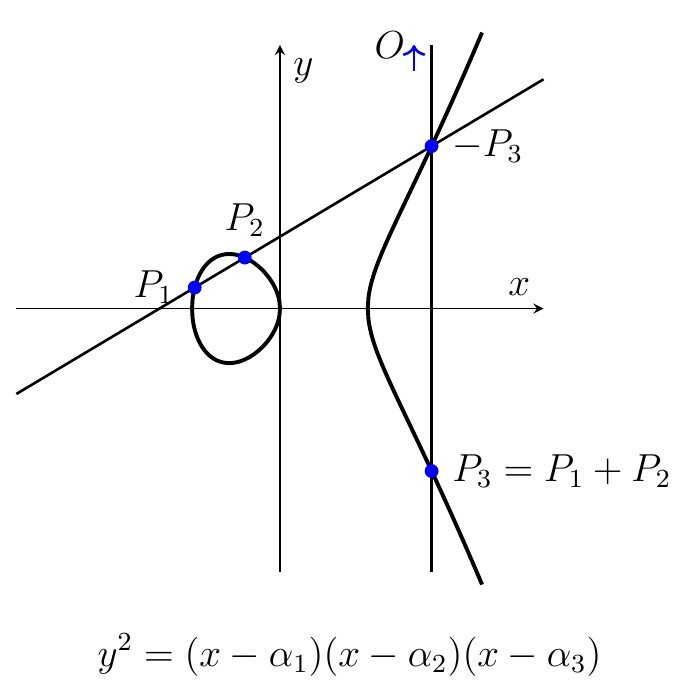
\includegraphics[width=.8\textwidth]{ellip1.jpg}
		\label{fig1}
	\end{minipage}
\end{figure}

\end{frame}
\section{算术几何基本定理}
\begin{frame}{目录}
\tableofcontents[currentsection]
\end{frame}
\begin{frame}[fragile]{陈述}
\begin{theorem}[Mordell定理]
	\hspace*{20pt}设$K$为数域,则椭圆曲线$E(K)$
	$$E/K:y^2=4x^3+g_2x+g_3 \qquad g_2,g_3 \in K$$
	关于上述群运算构成\CJKunderdot{有限生成}Abel群.
\end{theorem}
对Abel簇,同样有相同的结论:
\begin{theorem}[Mordell-Weil定理]
	\hspace*{20pt}设$K$为数域,则$K$上的Abel簇为\CJKunderdot{有限生成}Abel群.
\end{theorem}
\end{frame}
\begin{frame}[fragile]{证明概述}
\vspace{-1cm}
	\begin{figure}[th]
	\begin{minipage}[b]{\textwidth}
		\centering
		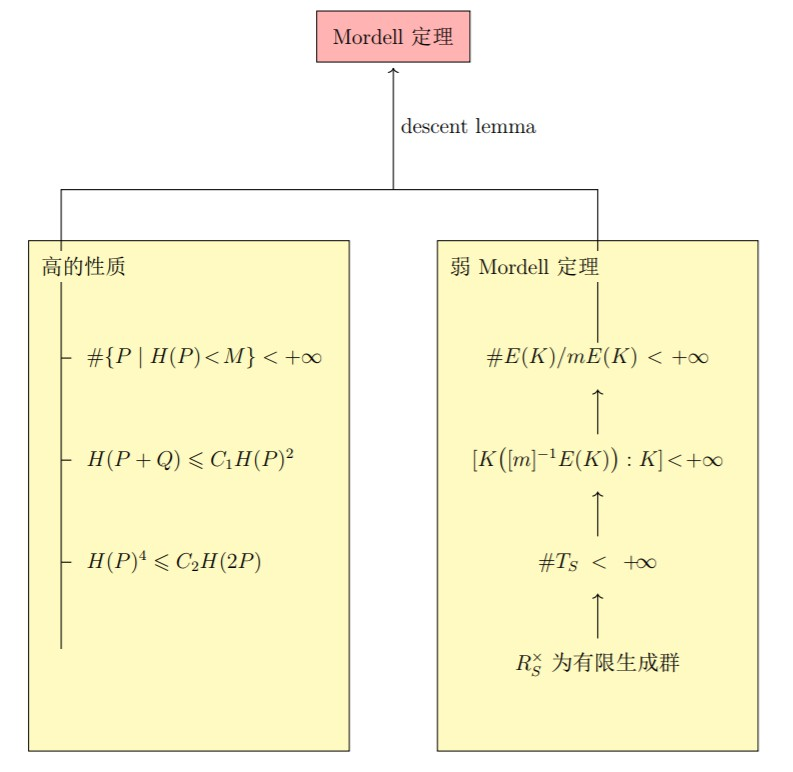
\includegraphics[width=0.72\textwidth]{mordell1.jpg}
		\label{fig2}
	\end{minipage}
\end{figure}
\end{frame}
\begin{frame}[fragile]{弱Modell定理}
\begin{theorem}[高的性质]
	\hspace*{20pt}设$K$为数域,则$E(K)/2E(K)$为\CJKunderdot{有限}群.
\end{theorem}
通过"x坐标"映射\begin{center}
	\begin{tikzcd}
		E(K)  \arrow[r, "\tilde{\varphi}_i"] & K^{\times} \arrow[r, "{\hat{\pi}}"]     & (K^{\times}/(K^{\times})^2)^3  \arrow[r, "{\hat{\eta}}"] & (P_K/(P_K)^2)^3   
	\end{tikzcd}
\end{center}
得到证明.
\begin{itemize}	
\item 用到理想类群与单位群的有限性.
\item 某些证明中用到了歧化理论.(局部与整体)
\item 引出: 
\begin{itemize}
	\item Galois上同调;
	\item Tamagawa数$c_v:=\#E(K_v)/E^0(K_v)$;
	\item m-Selmer群$S^{(m)}(E/K)$与Shafarevich-Tate群$\Sha(E/K)$.
\end{itemize}
\end{itemize}
\end{frame}
\begin{frame}[fragile]{高的性质}
\begin{defn}[Naive height]
	设$P=[x_0, \ldots, x_N] \in \mathbb{P}^N(K)$,定义$P$相对于$K$的高
	$$H_K(P)=\prod_{v \in M_K} \max \left\{|x_0|_v, \ldots , |x_N|_v \right\}^{n_v}$$
与椭圆曲线 $E/K$上的高
	$H_x(P)=H(x(P))$
\end{defn}
\begin{itemize}	
	\item 用到多项式的估计与乘积公式(定义);
	\item 引出: 
	\begin{itemize}
		\item \textbf{Néron-Tate height}:实线性空间$E(K) \otimes_{\mathbb{Z}}\mathbb{R}$上的一个内积;
		\item 无挠部分$\Lambda :=E(K)/E(K)_{\tor}$作为$E(K) \otimes_{\mathbb{Z}}\mathbb{R}$上的格点;
		\item 环面$E(K)\otimes_{\mathbb{Z}}\mathbb{R}/\Lambda$所对应的体积$R_{E/K}$.\\($r=0$时令$R_{E/K}=1$.)
	\end{itemize}
\end{itemize}
\end{frame}
\section{BSD猜想:简介}
\begin{frame}{目录}
\tableofcontents[currentsection]
\end{frame}
\begin{frame}[fragile]{同类数公式类比}
\begin{itemize}
	\item $\mathcal{O}_K^{\times} \longleftrightarrow E(\mathbb{Q})$:格点,对应的环面体积分别为$R_K$与$R_{E/\mathbb{Q}}$.
	$$\mathcal{O}_K^{\times}=H^0(K,\mathcal{O}_{\bar{K}}^{\times}) \qquad E(K)=H^0(K,E(\bar{K})).$$
	\item $Cl(K) \longleftrightarrow \Sha (E/\mathbb{Q})$:由于
	$$Cl(K):=\Ker \left\{H^1(K,\mathcal{O}_{\bar{K}}^{\times}) \longrightarrow \prod_{v}H^1(K_v,\mathcal{O}_{\bar{K}_v}^{\times}) \right\}$$
	$$\Sha(E/\mathbb{Q}):=\Ker \left\{H^1(\mathbb{Q},E(\bar{\mathbb{Q}})) \longrightarrow \prod_{v}H^1(\mathbb{Q}_v,E(\bar{\mathbb{Q}_v})) \right\}$$
	类群$Cl(K)$有限,$\Sha (E/\mathbb{Q})$有限?
	\item $\zeta_K(s) \longleftrightarrow L(E,s)$
\end{itemize}
\end{frame}
\begin{frame}[fragile]{$L$函数}
\begin{defn}[Hesse-Weil $L$函数]
	\hspace*{20pt}对素数$p$,考虑$E$模$p$的解的个数$N_p$(包含$O$),记$t_p:=p+1-N_p$,定义Hesse-Weil $L$函数
	$$L(E,s):=\prod_{p \mid \Delta} \frac{1}{1-t_pp^{-s}} \prod_{p \nmid \Delta} \frac{1}{1-t_pp^{-s}+p^{1-2s}}$$
\end{defn}
\end{frame}
\begin{frame}[fragile]{猜想陈述}
\begin{conj}[Birch and Swinnerton-Dyer Conjecture]
	\hspace*{20pt}对$\mathbb{Q}$上的椭圆曲线$E:y^2=x^3+Ax+B,\, A,B \in \mathbb{Z}$,我们有
	\begin{itemize}
		\item Hesse-Weil $L$函数在$1$点处的阶为椭圆曲线的秩$r_E$;
		\item Sha群$\Sha(E/\mathbb{Q})$有限;
		\item $$\hspace{-0.5cm}L(E,s)=\Omega(E)\!\! \prod_{p \text{ prime }}\hspace{-3mm}c_p(E)\cdot \#\Sha(E/\mathbb{Q})\frac{R_{E//\mathbb{Q}}}{(\#E(\mathbb{Q})_{\tor})^2} (s-1)^r$$
		$$\hspace{7cm}+O((s-1)^{r+1})$$
		其中$\Omega(E):=\int_{E(\mathbb{R})} \frac{dx}{2|y|}$为$E(\mathbb{R})$上的\textbf{N\'{e}ron周期}.
	\end{itemize}
\end{conj}
		%在这里,前半部分刻画了坏约化部分的影响,而后半部分则全然是类数公式的类比.(其中$\#E(\mathbb{Q}$取了平方是因为Hesse-Weil $L$函数是“2维”的)
\end{frame}
\begin{frame}[fragile]{进展}
\begin{itemize}
	\item Coates与Wiles(1977):对带复乘的椭圆曲线证明了了$L$-函数零点阶数为0(无零点)的情形.
	\item Benedict Gross与Don Zagier使用Gross-Zagier公式描绘了$L$-函数零点阶数为1的情形,随后被Kolyvagin用来说明
	$$\ord_{s=1}L(E,s)=1 \Longrightarrow r_E=1$$
	对部分秩为0或1的椭圆曲线(带有复乘且导子较小)证明了BSD猜想.
	\item 张伟与Christophe  Skinner等人通过对椭圆曲线的“计数”证明“至少有约$\frac{2}{3}$的椭圆曲线满足BSD猜想”.
\end{itemize}
\end{frame}
\begin{frame}[fragile]
Thank you!

\end{frame}
%%%%%%%%%%%%%%%%%%%%%%%%%%%%%%%%%%%%%%%%%%%%%%%%%%%%%%%%%%%%%%%%%%%%%%%%%%




%%%%%%%%%%%%%%%%%%%%%%%%%%%%%%%%%%%%%%%%%%%%%%%%%%%%%%%%%%%%%%%%%%%%%%%%%%%%%%%%%%%%%%%%%%%%%%%







\end{document}




